\documentclass{beamer}

%% Use package -----------------------------------------------------------------
\usepackage[T1]{fontenc}
\usepackage[utf8]{inputenc}
\usepackage{lmodern}
\usepackage{graphicx}
\usepackage[absolute,overlay]{textpos}
\usepackage{multicol}
\usepackage{listings}
\usepackage{svg}

%% Beamer customization---------------------------------------------------------

\usepackage{xcolor}
\usetheme{Warsaw}

%% Themes
% Outer themes
\useoutertheme{shadow}
% Rounded boxes and shadows
\useinnertheme[shadow=true]{rounded}
% Solid \item symbols
\useinnertheme{circles}

%% Custom colors
\definecolor{rltgreen}{rgb}{0,0.5,0}
\definecolor{pasteur}{RGB}{0,90,154}
\setbeamerfont{block title}{size={}}
\setbeamercolor{structure}{fg=pasteur}
\setbeamercolor{item}{fg=pasteur}

%Color of title
\setbeamertemplate{frametitle}
{
    \nointerlineskip
    \begin{beamercolorbox}[sep=0.3cm,ht=1.8em,wd=\paperwidth]{frametitle}
        \vbox{}\vskip-2ex%
        \strut\insertframetitle\strut
        \vskip-0.8ex%
    \end{beamercolorbox}
}
% Hide navigation symbols
\setbeamertemplate{navigation symbols}{}

%% Title block
\setbeamercolor*{title}{use=structure,fg=white,bg=pasteur}

\makeatletter

%% Top infolines
\setbeamertemplate{headline}{%
\leavevmode%
  \hbox{%
    \begin{beamercolorbox}[wd=\paperwidth,ht=2.5ex,dp=1.125ex]{palette quaternary}%
    \insertsectionnavigationhorizontal{\paperwidth}{}{\hskip0pt plus1filll}
    \end{beamercolorbox}%
  }
}

%% Define Snakemake ------------------------------------------------------------

\definecolor{eclipseBlue}{RGB}{42,0.0,255}
\definecolor{eclipseGreen}{RGB}{63,127,95}
\definecolor{eclipsePurple}{RGB}{127,0,85}

\lstset{language=Python}
\lstset{
    basicstyle=\tiny\ttfamily,
    morekeywords={rule, output, shell, params, run, configfile, temp},
    showstringspaces=false,
    commentstyle=\color{eclipseGreen}, % style of comments
    keywordstyle=\color{eclipsePurple}, % style of keywords
    stringstyle=\color{eclipseBlue}, % style of strings
}


%% Set up title ----------------------------------------------------------------

\title{Sequana in a nutshell}
\author[T.Cokelaer \& D.Desvillechabrol]{Thomas Cokelaer and Dimitri Desvillechabrol
and Rachel Legendre}
\institute{Institut Pasteur}
\date{Sept 20th 2016}



\AtBeginSection[]{
  \begin{frame}
  \vfill
  \centering
  \begin{beamercolorbox}[sep=8pt,center,shadow=true,rounded=true]{title}
    \usebeamerfont{title}\insertsectionhead\par%
  \end{beamercolorbox}
  \vfill
  \end{frame}
}

\begin{document}

%% Title slide -----------------------------------------------------------------

\begin{frame}[plain]
    \titlepage
    \begin{textblock*}{5cm}(4.5cm,0.3cm)
        
\includegraphics[scale=0.09]{images/Institut_Pasteur.png}
    \end{textblock*}
\end{frame}

%% Slides ----------------------------------------------------------------------

\section{Motivation}

\begin{frame}
 \frametitle{NGS at Biomics}
 
 Development driven by the Biomics Pole at Pasteur Institute, which involves
 many aspects of NGS including :
 
 \tiny
 \begin{block}{https://research.pasteur.fr/en/team/biomics/}
  \begin{itemize}
  \item De novo and targeted sequencing of viruses, prokaryotes and eukaryotes
  \item Variant (SNP, indel, large rearrangements) detection
  \item Human and Mouse SNP detection by array
  \item Transcriptional analysis (RNA-Seq) for both prokaryotes and eukaryotes
  \item 16S and deep-sequencing metagenomic studies (mouse, human, and other environments)
  \item Bottom-up whole proteomic analysis and quantification
  \item Analysis of a wide range of post-translational modifications
  \item Determination of the dynamics of protein complexes.
  \item Epigenetics (methylation studies)
  \item Projects involving two or more techniques (i.e. proteogenomics, single-cell DNA/RNA analysis)
  \end{itemize}
 \end{block}
 \small 
\end{frame}



\section{Sequana project}

\begin{frame}
    \frametitle{What is Sequana ?}
    \begin{block}{1. A Python library}
       \tiny
    \begin{itemize}
        \item Pandas for data mining, matplotlib for visualisation and the Python ecosystem (e.g., scikit-learn)
        \item Tools to simplify the interface with external dependencies (e.g., snpEff, kraken)
        \item More advanced NGS data structure (e.g., BAM reader with plotting functionalities)
    \end{itemize} 
    \end{block}
    \pause
    
    \begin{exampleblock}{2. A framework to store/design pipelines}
    \tiny
    \begin{itemize}
        \item Using Snakemake as a common language to design new pipelines
        \item Provide reusable snakemake rules and modules
    \end{itemize} 
     \end{exampleblock}
  \pause
  
    \begin{block}{3. A set of HTML reports}
    \tiny
    \begin{itemize}
	\item We use JINJA templating to re-use HTML templates
    \end{itemize} 
    \end{block}
  \pause  
    \begin{block}{4. A suite of standalone applications}
    \tiny
    \begin{itemize}
	\item sequana (create pipeline and config file locally)
	\item sequana\_coverage
	\item sequana\_mapping
	\item \dots
    \end{itemize} 
    \end{block}
\end{frame}

\begin{frame}[fragile]
    \frametitle{1. A Python library: example}
    \begin{block}{}
    \begin{lstlisting}
     from sequana import BAM, sequana_data
     datatest = sequana_data('test.bam', "testing")

     # Use sequana.bamtools.BAM class to plot the MAPQ histogram
     b = BAM(datatest)
     b.plot_bar_mapq()
    \end{lstlisting}
    \end{block}
    \centering{
        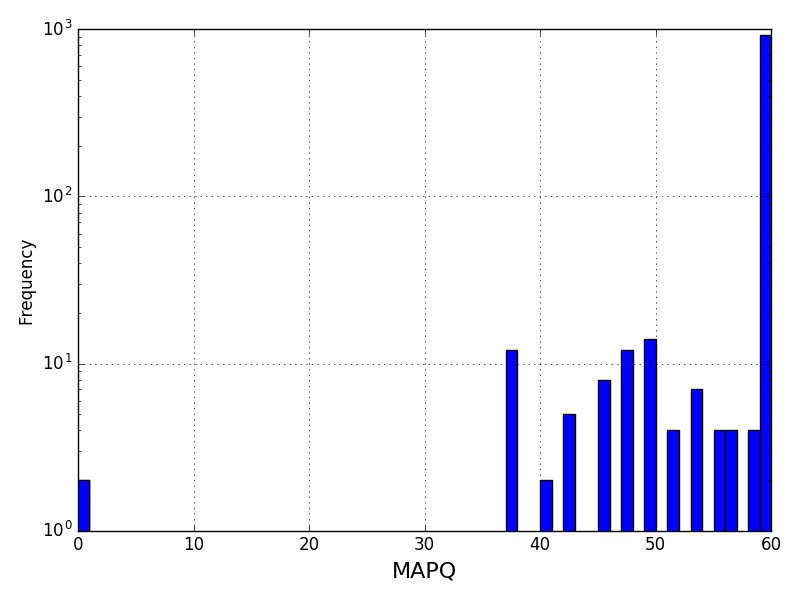
\includegraphics[scale=0.35]{images/mapq.png}
    }
    
\end{frame}    
    

\begin{frame}[fragile]
    \frametitle{2. A framework to design pipelines}
    \tiny
    We currently have 4 end-user pipelines in snakemake format:
    \begin{block}{}
    \begin{itemize}
      \item quality\_taxon: phix removal + trimming (quality, adapters) + taxonomy
      \item variant\_calling: detection of variant  using FreeBayes
      \item denovo\_assembly: denovo assembly + coverage of the contigs + variant calling
      \item compressor: utility to convert FastQ recursively between different compression formats
    \end{itemize}
    
    \end{block}
    and about 40 rules. 
    
    \begin{minipage}{100pc}
            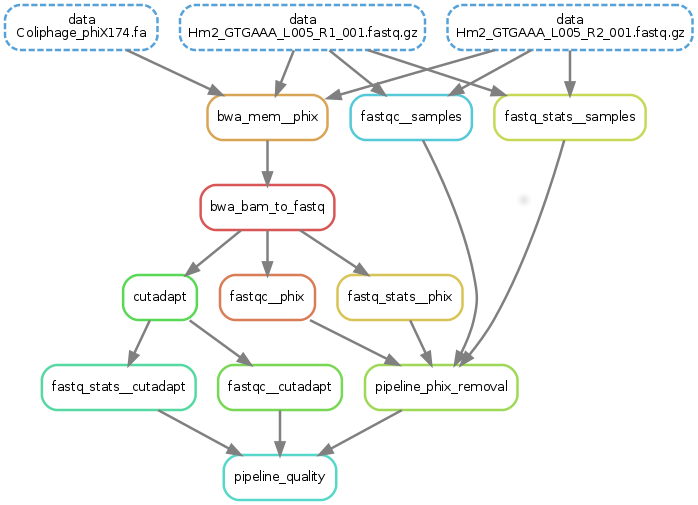
\includegraphics[scale=0.30]{images/quality_dag.png}
            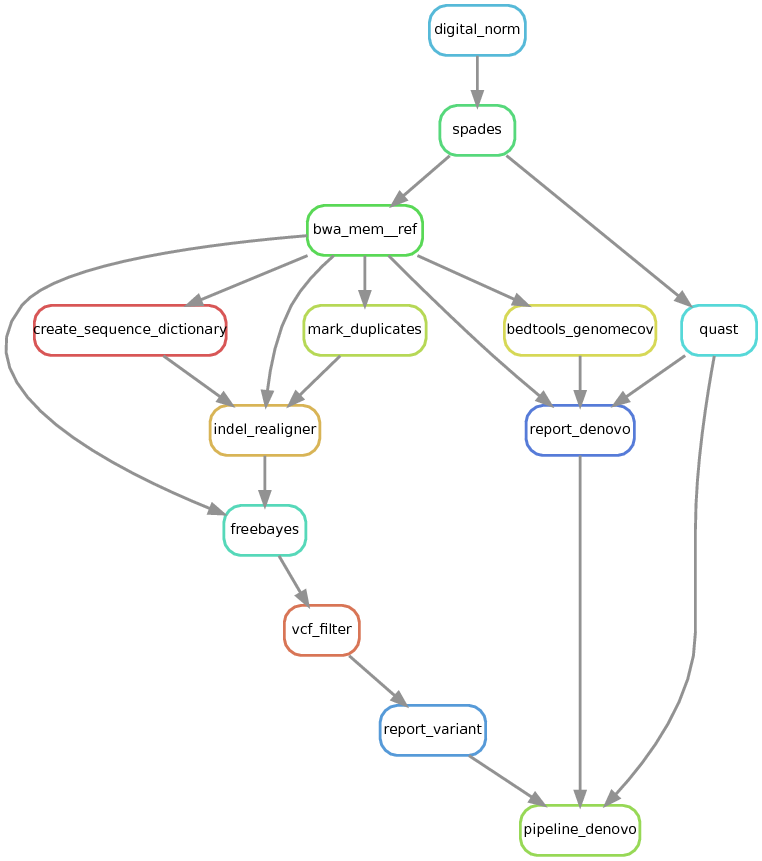
\includegraphics[scale=0.15]{images/denovo_dag.png}
    \end{minipage}

\end{frame}


\begin{frame}[fragile]
    \frametitle{3. Reporting}
    Each pipeline is associated with a HTML report. Reports can be re-used 
    outside of the pipelines (for instance in standalone app)
    \begin{block}{Inside a Snakefile}
    \begin{lstlisting}
    rule report:
    input:
        dag = "dag.svg"
    output: "report/index.html"
    run:
        from sequana import report_main
        s = report_main.SequanaReport()
        s.create_report()
    \end{lstlisting}
    \end{block}
    
    \begin{block}{JINJA template}
    \begin{lstlisting}
    
    
      <div class="section" id="Input">
        <h2> 1 -  <a class="toc-backref" href="#id1">Input</a></h2>
        <a href=""> </a>
         The BAM file contains {{ alignment_count }} fragments/alignments.
      </div>
    
  \end{lstlisting}
   \end{block}

 
\end{frame}



\begin{frame}[fragile]
    \frametitle{4. Standalone}
    
    \begin{itemize}
     \item sequana: creates a config and pipeline locally ready to use.
     \item sequana\_coverage: standalone for the coverage (mapping) 
     \item sequana\_mapping:  a quick mapping on a reference
     \item sequana\_summary: summary for multiple sequana projects, or to get inforamtion about a specific set of input file(s), e.g. fastq)
     \item sequana\_taxonomy (standalone to use kraken/krona)   
     \item sequana\_compressor  (in progress, a snakefile rule)
    \end{itemize}   
\end{frame}



\section{snakefile design and choices}

\begin{frame}[fragile]
    \frametitle{snakefile storage}
    Snakefiles are stored in the ./pipelines or ./rules directories and their path
    can be retrieved automatically.
    \tiny
    \begin{block}{Snakefile storage and metadata}
    \begin{lstlisting}
     >>> from sequana import snaketools 
     >>> snaketools.rules.keys()
     ['bwa_mem_dynamic', 'cutadapt', 'dag', 'report_variant' ...
     >>> m = snaketools.Module('quality_taxon')
     >>> m.overview
     "Quality pipeline and taxonomic search"
     >>> m.config
     ".../sequana/pipelines/quality_pipeline/Snakefile"
    \end{lstlisting}

    You can include them in other snakefiles using e.g. :
    \begin{lstlisting}
    import sequana.snaketools as sequana
    include: sequana.modules['dag']
    include: sequana.modules['variants']
    \end{lstlisting}

    \end{block}
\end{frame}


\begin{frame}[fragile]
 \frametitle{config file}
 Each pipeline include a config file. We could use json or yaml and decided 
 to go for yaml, which is a bit easier to handle for end-users.
 
\begin{block}{}
 \begin{lstlisting} 
# list of your input file
samples:
    file1: "%(file1)s"
    file2: "%(file2)s"

project: "%(project)s"

# if files are required for a pipeline and are within sequana or should
# # be downloaded before the pipeline provide them in this section
# # Note that sequana and url fields are followed by itemised files or links
# using# the front dashes
requirements:
    - phiX174.fa

# =========================================== For testing only
fastq_sampling:
    do: no
    N: 100000
\end{lstlisting}
\end{block}
 
 \small

The config file are \textit{templatized} and each rule has its own section.
Or, each section has its own rule except for samples, project and requirements 
sections.
\end{frame}


\begin{frame}
 \frametitle{snakefile own rules}
 \tiny
 \begin{block}{}
  \begin{itemize}
   \item No expand except in the first rule so that the pipeline can be 
     re-run (far more easier for debugging)
   \item pipelines and rules are stored in their own directory, named after the rule. 
   the filename is named after the rule as well with the ``.rulers'' extension.
   \item In our terminology, a rule is a snakefile that is self-content while
   a pipeline is a snakefile that includes other snakefiles/rules. They are stored
   in different directories (pipelines/ and rules/)
   \item In the directory of a pipeline (or rule), one can add a dedicated config 
   file and a README. By default the config file at the root of the directory is 
   used, otherwise the local config file is used.
   \item We used \textit{dynamic rules}
   \item Optional rules have a \textbf{do} field in the config file
   \end{itemize}
 \end{block} 
\end{frame}



\begin{frame}
\frametitle{snaketools}
 \begin{block}{}
 \begin{itemize}
  \item SequanaConfig: read a config file and performs sanity checks
  \item ExpandedSnakefile: reads a pipeline (with includes) and returns a full version
  without includes.
  \item SnakeMakeStats: read the stats file and create a plot
  \item Module: handler for a rule or pipeline
  \item DotParser
  \item FastQFactory: gives easy access to paths, filenames, basenames, extensions, ...
  \end{itemize}
 \end{block} 
\end{frame}


\begin{frame}
 \frametitle{others}
 \begin{block}{}
 \begin{itemize}
  \item Name of the snakefile is stored in a local \_\_snakefile\_\_ variable, which can be
 used in rules that are included later on.
 \item pipeline can include pipeline
 \item abstract input and output in the rules
 \end{itemize}
 \end{block}
\end{frame}




\section{Continuous integration}

\begin{frame}[fragile]
 \frametitle{Versioning}
Sequana is available on github (github.com/sequana/sequana)

About 1000 commits \\
\begin{center}
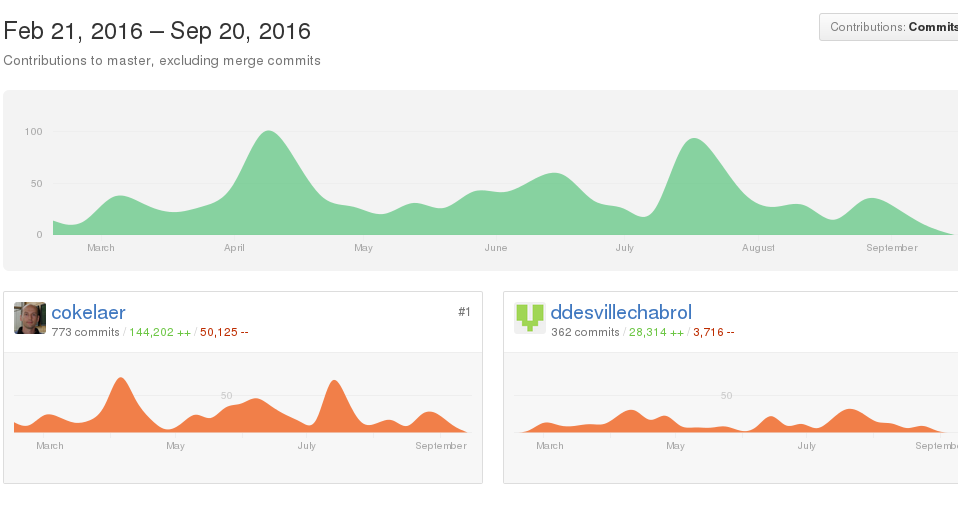
\includegraphics[scale=0.2]{images/commits}
\end{center}
260 issues (15 open).

\end{frame}



\begin{frame}[fragile]
    \frametitle{test suite}
    \begin{block}{}
    Continuous Integration on Travis with 60 tests with 60\% coverage
    \end{block}
    
    
    %\begin{textblock*}{7cm}(.5cm,3.5cm)
        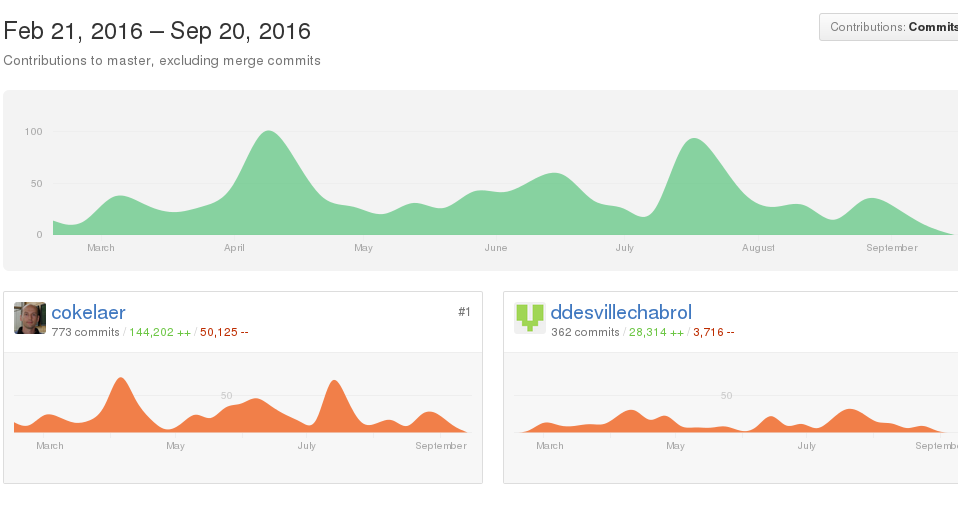
\includegraphics[scale=0.35]{images/commits}
    %\end{textblock*}
\end{frame}


\begin{frame}[fragile]
    \frametitle{Documentation}
    Fully documented and available on RTD: sequana.readthedocs.org
    Uses Sphinx to documented the source code and provide user guide.
    Updated automatically at each commits on the master branch.
\begin{center}
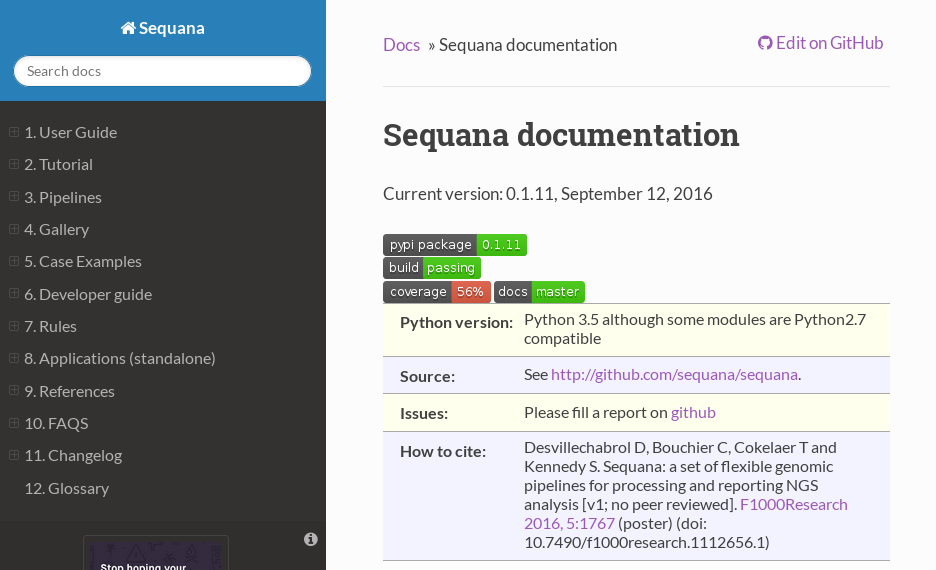
\includegraphics[scale=0.3]{images/rtd}
\end{center}
    
\end{frame}


\section{Future Directions}

\begin{frame}
\begin{block}{Pipelines to come}
\begin{itemize}
 \item PacBio was acquired recently. Therefore the next logical pipeline is to include
 a long reads pipeline (TC, DD). 
 \item Epigenomics
     \begin{itemize}
     \item Methylation
      \item Chip-seq 
      \item atac-seq 
     \end{itemize}
 \item RNA-related projects (RL)
     \begin{itemize}
     \item Portage of existing RNA-seq pipeline into a snakemake-framework
     \item miRNA / RIBO-seq   
     \end{itemize}
\end{itemize}
\end{block}

\begin{block}{Future developments}
 \begin{itemize}
  \item GUI 
  \item Docker
 \end{itemize}
\end{block}
 \end{frame}

\end{document}
